\section{Experimentos e Resultados}
\label{sec:experimentos}

\subsection{Ambiente de Execução e Organização das Baterias}
\label{sec:ambiente}

Todas as baterias rodaram na plataforma Flautim, em contêineres com 6 núcleos de CPU, 16~GB de
RAM e uma fatia MIG \texttt{1g.18gb} de uma GPU NVIDIA H200, sob Python~3.11. Cada caso do
\textit{Branch-and-Bound} executou em subprocesso próprio (Seção~\ref{sec:instrumentacao}), com
três casos simultâneos por contêiner e teto de 4~GiB de memória por caso. Dividimos o estudo em
quatro baterias:

\begin{itemize}
  \item \textbf{A (algoritmos polinomiais)}: \textit{Twice-Around-The-Tree} e Christofides nas
  versões \texttt{v0} e \texttt{v1}, mais as heurísticas de \textit{warm-start}, nas 15
  instâncias. Os tempos são a mediana de 5 repetições.
  \item \textbf{B (evolução do \textit{Branch-and-Bound})}: as versões \texttt{v0}--\texttt{v3}
  com \textit{Cold Start} e com Christofides, limite de 120~s por caso.
  \item \textbf{C (\textit{warm-starts})}: a versão \texttt{v3} com as cinco estratégias de
  inicialização, limite de 30 minutos por caso.
  \item \textbf{D (GPU)}: as versões \texttt{v1}--\texttt{v3} com e sem a \textit{flag}
  \texttt{--use-gpu}, limite de 300~s; a \texttt{v1} foi medida com lotes de 128 e 1024 pais.
\end{itemize}

Nas tabelas, \texttt{TL} indica que o caso atingiu o limite de tempo sem provar o ótimo, e
\texttt{OOM}, que atingiu o teto de memória. Quando há gap entre parênteses, ele é o erro
relativo da melhor rota encontrada até a parada.

Durante as primeiras execuções, a \texttt{v1} travava ao se aproximar do teto de memória: o
processo ficava preso no tratamento da exceção e era encerrado sem registrar resultado. Na GPU
não havia teto algum, e a fila chegou a ocupar 16,6~GB. Para que CPU e GPU fossem comparadas
nas mesmas condições, a \texttt{v1} passou a verificar o próprio pico de memória residente a
cada 16 iterações e a encerrar com estado \texttt{OOM} ao chegar a 256~MB do teto. Todas as
linhas da \texttt{v1} apresentadas aqui vêm dessa versão corrigida.

\subsection{Bateria A: Algoritmos Aproximados e Complexidade Empírica}
\label{sec:res_aproximados}

\paragraph{Ganho das refatorações (\texttt{v0} $\rightarrow$ \texttt{v1}).}
No \textit{Twice-Around-The-Tree}, a troca do grafo completo em dicionários por matrizes densas
derrubou o pico de memória de 655~KiB para 4,1~KiB em \texttt{st70} ($N = 70$), e o tempo de
12,2~ms para 0,29~ms. A memória da \texttt{v0} segue de perto a curva quadrática
($R^2 = 0{,}997$, Figura~\ref{fig:complexidade}), enquanto a da \texttt{v1} é linear
($R^2 = 0{,}996$), o que confirma o item (i) de $H_{TA}$. No Christofides o ganho é menor: o
pico caiu de 655~KiB para 341~KiB e o tempo, de 35,0~ms para 16,5~ms, porque o emparelhamento
Blossom, que não mudou entre as versões, responde por 91,5\% do tempo total da \texttt{v1} e por
todo o seu pico de memória (Figura~\ref{fig:profiling}). Esse pico acompanha $|I|$, e não $N$:
\texttt{att48}, com 30 vértices ímpares, consome mais memória que \texttt{berlin52}, com 22.

\includeFigIfExists{figures/fig1_subroutine_profiling.pdf}
{Bateria A. À esquerda, tempo mediano do Christofides \texttt{v1} por subrotina; à direita, pico
de memória das versões \texttt{v0} e \texttt{v1} dos dois algoritmos aproximados. As curvas das
duas \texttt{v0} se sobrepõem porque ambas constroem o mesmo grafo completo.}
{fig:profiling}
{Gerada por \texttt{python -m src.cli analyze}.}

\paragraph{Aderência aos modelos teóricos.}
A Tabela~\ref{tab:ajustes} resume os ajustes. As séries de memória aderem quase perfeitamente
aos modelos previstos. As de tempo variam mais, e o motivo é a escala: o Prim denso leva entre
0,08 e 0,65~ms, a travessia em pré-ordem e o Hierholzer ficam abaixo de 0,1~ms, e nessa faixa
o custo fixo do interpretador e a variação do escalonador pesam tanto quanto o termo
assintótico. Com $N \le 70$, o termo quadrático do Prim ainda não domina o tempo medido, e daí
os valores baixos de $R^2$ (0,34 no \textit{Twice-Around-The-Tree} e 0,57 no Christofides).
Restringimos os coeficientes de crescimento dos ajustes a valores não negativos, já que sem
essa restrição o ruído gerava parábolas côncavas, sem sentido para um custo computacional. No
emparelhamento, o ajuste cúbico em $|I|$ atinge $R^2 = 0{,}875$, contra $0{,}663$ do ajuste
cúbico em $N$, e a memória do Blossom em função de $|I|^2$ chega a $R^2 = 0{,}999$. Isso confirma os itens (ii) e (iii) de
$H_C$: o custo do Christofides é governado pelo número de vértices ímpares da AGM. Entre as
heurísticas de \textit{warm-start}, a inserção mais barata refatorada se ajusta razoavelmente a
$N^2 \log N$ ($R^2 = 0{,}71$). A Varredura de Graham, com tempos de centésimos de milissegundo,
não permite conclusão ($R^2 = 0{,}32$), de modo que o item (i) de $H_W$ fica apenas
parcialmente sustentado.

\begin{table}[htbp]
  \centering
  \caption{Ajustes de complexidade empírica selecionados (Bateria A, 15 instâncias). Coeficientes
  de crescimento restritos a valores não negativos.}
  \label{tab:ajustes}
  \small
  \begin{tabular}{llllr}
    \toprule
    Algoritmo & Métrica & Variável & Modelo & $R^2$ \\
    \midrule
    \textit{Twice-Around} \texttt{v0} & memória do grafo & $N$ & $N^2$ & 0,997 \\
    \textit{Twice-Around} \texttt{v1} & memória total & $N$ & $N$ & 0,996 \\
    \textit{Twice-Around} \texttt{v1} & tempo do Prim & $N$ & $N^2$ & 0,342 \\
    \textit{Twice-Around} \texttt{v1} & tempo da pré-ordem & $N$ & $N$ & 0,214 \\
    Christofides \texttt{v1} & tempo do Prim & $N$ & $N^2$ & 0,568 \\
    Christofides \texttt{v1} & tempo do Hierholzer & $N$ & $N$ & 0,380 \\
    Christofides \texttt{v1} & tempo do Blossom & $N$ & $N^3$ & 0,663 \\
    Christofides \texttt{v1} & tempo do Blossom & $|I|$ & $|I|^3$ & 0,875 \\
    Christofides \texttt{v1} & memória do Blossom & $|I|$ & $|I|^2$ & 0,999 \\
    Fecho Convexo & tempo da inserção & $N$ & $N^2 \log N$ & 0,714 \\
    Fecho Convexo & tempo de Graham & $N$ & $N \log N$ & 0,321 \\
    \bottomrule
  \end{tabular}
\end{table}

\includeFigIfExists{figures/fig2_complexity_regression.pdf}
{Bateria A. Pontos medidos e curvas teóricas ajustadas para o Prim denso, o emparelhamento
Blossom (em função de $|I|$), a memória do grafo completo na \texttt{v0} e a inserção mais
barata do Fecho Convexo.}
{fig:complexidade}
{Gerada por \texttt{python -m src.cli analyze}.}

\paragraph{Qualidade das soluções.}
A Tabela~\ref{tab:gaps} mostra o erro relativo de cada heurística em relação ao ótimo
certificado pelo oráculo. As garantias teóricas valem com folga: o maior erro do Christofides
foi 15,5\% (\texttt{eil51\_n18}), longe dos 50\% permitidos, e o do \textit{Twice-Around-The-Tree}
foi 47,1\% (\texttt{eil51\_n38}), abaixo dos 100\%. O \textit{Twice-Around-The-Tree} perdeu do
Christofides nas 15 instâncias (erro médio de 26,2\% contra 7,4\%), como previa o item (iii) de
$H_{TA}$. Ele também perdeu do Vizinho Mais Próximo, que não tem garantia nenhuma, em 12 das 15
instâncias (média de 16,4\%). A Inserção em Fecho Convexo foi a melhor em 14 das 15 instâncias,
com erro médio de 2,2\%, e chegou ao ótimo em quatro delas. A única exceção foi
\texttt{ulysses16}, onde o Christofides ficou em 1,2\% e o Fecho Convexo, em 1,5\%.

\includeTableIfExists{tables/tab_approx_gaps.tex}
{Erro relativo (\%) das heurísticas em relação ao ótimo \texttt{EUC\_2D} certificado.}
{tab:gaps}
{Gerada por \texttt{python -m src.cli analyze}.}

\subsection{Bateria B: Evolução Gradual do \textit{Branch-and-Bound}}
\label{sec:res_bnb}

A Tabela~\ref{tab:ablacao} e a Figura~\ref{fig:ablacao} mostram as quatro versões lado a lado.
Com limite de 120~s, as versões \texttt{v0}, \texttt{v1} e \texttt{v2} resolveram as mesmas
quatro instâncias (\texttt{eil51\_n10}, \texttt{berlin52\_n12}, \texttt{burma14} e
\texttt{eil51\_n18}); a \texttt{v3} resolveu também \texttt{berlin52\_n20}, em 80~s. Nas
demais, cada versão parou por um motivo diferente.

\includeTableIfExists{tables/tab_bnb_ablation.tex}
{Bateria B. Tempo (s) até provar o ótimo, por versão e inicialização (Frio = \textit{Cold Start};
Chr. = Christofides). Limite de 120~s por caso.}
{tab:ablacao}
{Gerada por \texttt{python -m src.cli analyze}.}

\paragraph{$H_0$ (\texttt{v0\_naive}).}
A \texttt{v0} processou uma mediana de cerca de 1\,000 nós por segundo. Como cada expansão custa
$O(N^3)$, a vazão desaba com $N$: em \texttt{st70} ela expandiu apenas 4\,416 nós em 120~s. Por
isso a \texttt{v0} nunca chegou ao teto de memória. A fila atingiu no máximo 2,7 milhões de
estados (948~MB), e o tempo acabou antes. A hipótese se confirma pelo lado do tempo; o colapso
por memória previsto não ocorreu nesse limite de 120~s porque a própria lentidão da versão
impediu a fila de crescer. Sem um bom incumbente, a rota final após o limite ficou em mediana
176\% acima do ótimo com \textit{Cold Start}.

\paragraph{$H_1$ (\texttt{v1\_gpu}).}
O cálculo vetorizado do limite elevou a vazão mediana para 24\,000 nós/s, 23 vezes a da
\texttt{v0}. Nas instâncias resolvidas, o tempo caiu na mesma proporção (\texttt{burma14}: de
64~s para 4,4~s). A memória, porém, continuou exponencial: a fila \textit{Best-First} chegou a
cerca de $10^7$ estados, e a \texttt{v1} atingiu o teto de 4~GiB nas 11 instâncias restantes,
sempre entre 28 e 69~s de execução. A expansão especulativa em lote só apareceu na menor
instância (\texttt{eil51\_n10}: 853 nós contra 194 da \texttt{v0}); de $N = 12$ em diante, a
diferença foi de poucos nós. Os resultados confirmam $H_1$ inteira: a \texttt{v1} ficou mais
rápida e, justamente por isso, esgotou a memória mais cedo.

\includeFigIfExists{figures/fig3_bnb_gradual_optimization.pdf}
{Bateria B com \textit{Cold Start}. À esquerda, tempo até o término (barras hachuradas pararam
no limite de tempo ou de memória); à direita, pico de nós simultâneos na fila ou na pilha.}
{fig:ablacao}
{Gerada por \texttt{python -m src.cli analyze}.}

\paragraph{$H_2$ (\texttt{v2\_dfs\_memory}).}
A troca para DFS eliminou os OOMs. A pilha nunca passou de $N$ estados (70 em \texttt{st70}),
contra os $10^6$ a $10^7$ das versões com fila, e o pico de memória do processo ficou em
196~MB, quase todo consumido pelo próprio interpretador e pelas bibliotecas. A questão aberta
em $H_2$ teve resposta negativa: a vazão subiu só para 50\,000 nós/s, porque cada nó ainda
aloca pequenos vetores. A DFS também expande mais nós que a busca \textit{Best-First}, que por
construção expande o menor número possível (\texttt{eil51\_n18}: 170\,517 nós contra
106\,773). Com as duas coisas somadas, a \texttt{v2} foi mais lenta que a \texttt{v1} em todas
as instâncias que ambas resolveram (\texttt{burma14}: 9,5~s contra 4,4~s).

\paragraph{$H_3$ (\texttt{v3\_fast\_bound}).}
O cálculo escalar do limite e o \textit{bitmask} multiplicaram a vazão por oito em relação à
\texttt{v2}, chegando a 420\,000 nós/s, a maior entre as versões. Isso bastou para resolver
\texttt{berlin52\_n20} e para deixar as rotas incumbentes mais próximas do ótimo ao fim do
limite (gap mediano de 7,7\% com \textit{Cold Start}). A redução de nós pela quebra de simetria
ficou bem abaixo da metade prevista. Em \texttt{burma14} e \texttt{berlin52\_n12}, a
\texttt{v3} expandiu de 6\% a 16\% menos nós que a \texttt{v2}. Em \texttt{eil51\_n18}, expandiu
quase três vezes mais (502\,256 contra 170\,517). É o efeito de atraso que anunciamos na
Seção~\ref{sec:bnb_versoes}: ao proibir uma das orientações, a busca pode demorar mais a achar
um bom incumbente. O efeito aparece também com Christofides, cujo $UB_0$ fica 15,5\% acima do
ótimo nessa instância e portanto não chega a ser apertado. Mesmo assim, a \texttt{v3} foi a
versão mais rápida em todas as instâncias resolvidas, porque a vazão maior compensa os nós
extras.

Nesta bateria, iniciar com Christofides em vez de \textit{Cold Start} quase não alterou os
tempos; a Bateria C explica o motivo.

\subsection{Bateria C: Impacto dos \textit{Warm-Starts}}
\label{sec:res_warmstart}

Com 30 minutos por caso, a \texttt{v3} provou o ótimo com qualquer inicialização nas sete
instâncias de $N \le 25$, exceto \texttt{ulysses22}, e em nenhuma das maiores
(Tabela~\ref{tab:warmstart}). O custo das próprias heurísticas foi desprezível: o mais caro, o
Christofides, levou no máximo 29~ms, e o Fecho Convexo, 4~ms, enquanto as buscas duraram de
segundos a minutos. O que diferencia as estratégias é o tamanho da árvore que cada $UB_0$ deixa
para explorar.

\includeTableIfExists{tables/tab_bnb_warmstart.tex}
{Bateria C (\texttt{v3}, limite de 30 minutos). Tempo total (s) até provar o ótimo; em
\texttt{TL}, o gap da melhor rota encontrada.}
{tab:warmstart}
{Gerada por \texttt{python -m src.cli analyze}.}

Em média, Vizinho Mais Próximo e \textit{Twice-Around-The-Tree} reduziram a árvore em 0,1\% e
0,0\%, o Christofides em 3,4\% e o Fecho Convexo em 41,5\% (Figura~\ref{fig:warmstart}). Em
\texttt{eil51\_n25}, o Fecho Convexo baixou a contagem de 206 milhões de nós para 14 milhões, e
o tempo, de 341~s para 26~s. Como a DFS da \texttt{v3} desce primeiro pelos filhos de menor
limite inferior, ela chega cedo a uma folha e tem um incumbente razoável mesmo partindo do frio.
Um $UB_0$ só muda a poda quando já é melhor que esse primeiro incumbente. As rotas do Vizinho
Mais Próximo (5\% a 42\% acima do ótimo) e do \textit{Twice-Around-The-Tree} (8\% a 47\%) não
costumam ser; as do Fecho Convexo (0\% a 7,4\%) costumam.

\includeFigIfExists{figures/fig4_warmstart_tradeoff.pdf}
{Bateria C. À esquerda, redução média de nós expandidos em relação ao \textit{Cold Start}; à
direita, nós expandidos por instância. Apenas as sete instâncias resolvidas por todas as
estratégias entram na comparação.}
{fig:warmstart}
{Gerada por \texttt{python -m src.cli analyze}.}

Nas instâncias que estouraram o limite, a inicialização define a qualidade da resposta. Em
\texttt{st70}, as partidas fria, por Vizinho Mais Próximo e por \textit{Twice-Around-The-Tree}
terminaram todas na mesma rota, 18,6\% acima do ótimo. Christofides e Fecho Convexo terminaram
com 9,1\% e 4,5\%, exatamente os erros de suas rotas iniciais: em 30 minutos, a busca não
encontrou nada melhor que elas. O item (ii) de $H_W$ se confirma para o Fecho Convexo e,
de forma muito mais modesta, para o Christofides, que preserva estrutura global, mas parte de
rotas de 1\% a 15\% acima do ótimo.

\subsection{Sensibilidade Topológica e Instâncias Adversariais}
\label{sec:res_sensibilidade}

O fator que mais pesou no esforço da busca exata foi a qualidade do limite inferior na raiz, e
ela depende da distribuição espacial dos pontos. A razão entre o limite de grau 2 na raiz e o
ótimo variou de 0,639 (\texttt{ulysses22}) a 0,936 (\texttt{eil51\_n38}). O gap desse limite
correlaciona-se fortemente com o coeficiente de variação das distâncias ao vizinho mais próximo
(Spearman $\rho = 0{,}90$) e das arestas da AGM ($\rho = 0{,}90$), e negativamente com a entropia
espacial ($\rho = -0{,}81$). Instâncias com aglomerados e pontos isolados, como as
\texttt{ulysses} e os recortes de \texttt{berlin52}, enfraquecem o limite, e pontos espalhados de
modo uniforme, como os de \texttt{eil51}, o mantêm apertado (Figura~\ref{fig:sensibilidade}). \texttt{ulysses16} tem menos vértices que
\texttt{eil51\_n18}, mas exigiu 340 vezes mais nós (170 milhões contra 500 mil) e 325~s contra
1,6~s.

\includeFigIfExists{figures/fig5_sensitivity_analysis.pdf}
{À esquerda, coeficientes padronizados da regressão Ridge para o erro dos dois algoritmos com
garantia. Ao centro e à direita, uma instância regular e uma adversarial, com a razão entre o
limite inferior na raiz e o ótimo e o tempo do \textit{Branch-and-Bound} com \textit{Cold Start}.}
{fig:sensibilidade}
{Gerada por \texttt{python -m src.cli analyze}.}

Quanto às heurísticas, o erro do Fecho Convexo diminui à medida que mais pontos pertencem à
envoltória ($\rho = -0{,}70$), o que é coerente com o seu funcionamento: quanto maior o fecho
inicial, menos inserções restam. O erro do \textit{Twice-Around-The-Tree} cresce com a entropia
espacial ($\rho = 0{,}67$), e o do Christofides não tem nenhuma correlação forte com os
descritores (todas abaixo de 0,47 em módulo), o que se espera de um algoritmo com garantia
apertada. A previsão de $H_{TA}$ de que vértices de grau alto na AGM piorariam o
\textit{Twice-Around-The-Tree} não se sustentou ($\rho = 0{,}03$). Esses números vêm de apenas 15
instâncias, com descritores correlacionados entre si, e devem ser lidos como tendências.

\subsection{Bateria D: Validação da Aceleração em GPU}
\label{sec:res_gpu}

A GPU não acelerou nenhuma versão (Figura~\ref{fig:gpu}). Nas instâncias pequenas, ela atrasou
a execução: em \texttt{eil51\_n10}, a \texttt{v1} levou 2,1~s na GPU contra 4~ms na CPU, quase
todo esse tempo gasto inicializando o contexto CUDA e transferindo dados. Lotes maiores
amortizam parte desse custo (0,26~s com lote de 1024). Nas instâncias que vão até o limite, a
vazão em nós por segundo foi praticamente a mesma nos dois dispositivos: a razão GPU/CPU teve
mediana entre 0,89 e 0,99 nas quatro configurações. Isso é coerente com o projeto: na
\texttt{v2} e na \texttt{v3} a GPU atua apenas na fronteira do nível 2, e toda a DFS roda na
CPU; na \texttt{v1}, um lote de até 1024 pais gera algumas dezenas de milhares de candidatos,
pouco para ocupar a GPU, e a fila continua sendo manipulada na CPU. Com o teto de memória
igual nos dois lados, a \texttt{v1} esgotou os 4~GiB exatamente nas mesmas 11 instâncias, em CPU
e em GPU. Nesse regime de $N \le 70$, o gargalo é a explosão combinatória da árvore e o custo
por nó no interpretador, e não a aritmética do limite inferior.

\begin{figure}[htbp]
  \centering
  \IfFileExists{figures/fig6_gpu_validation.pdf}{%
    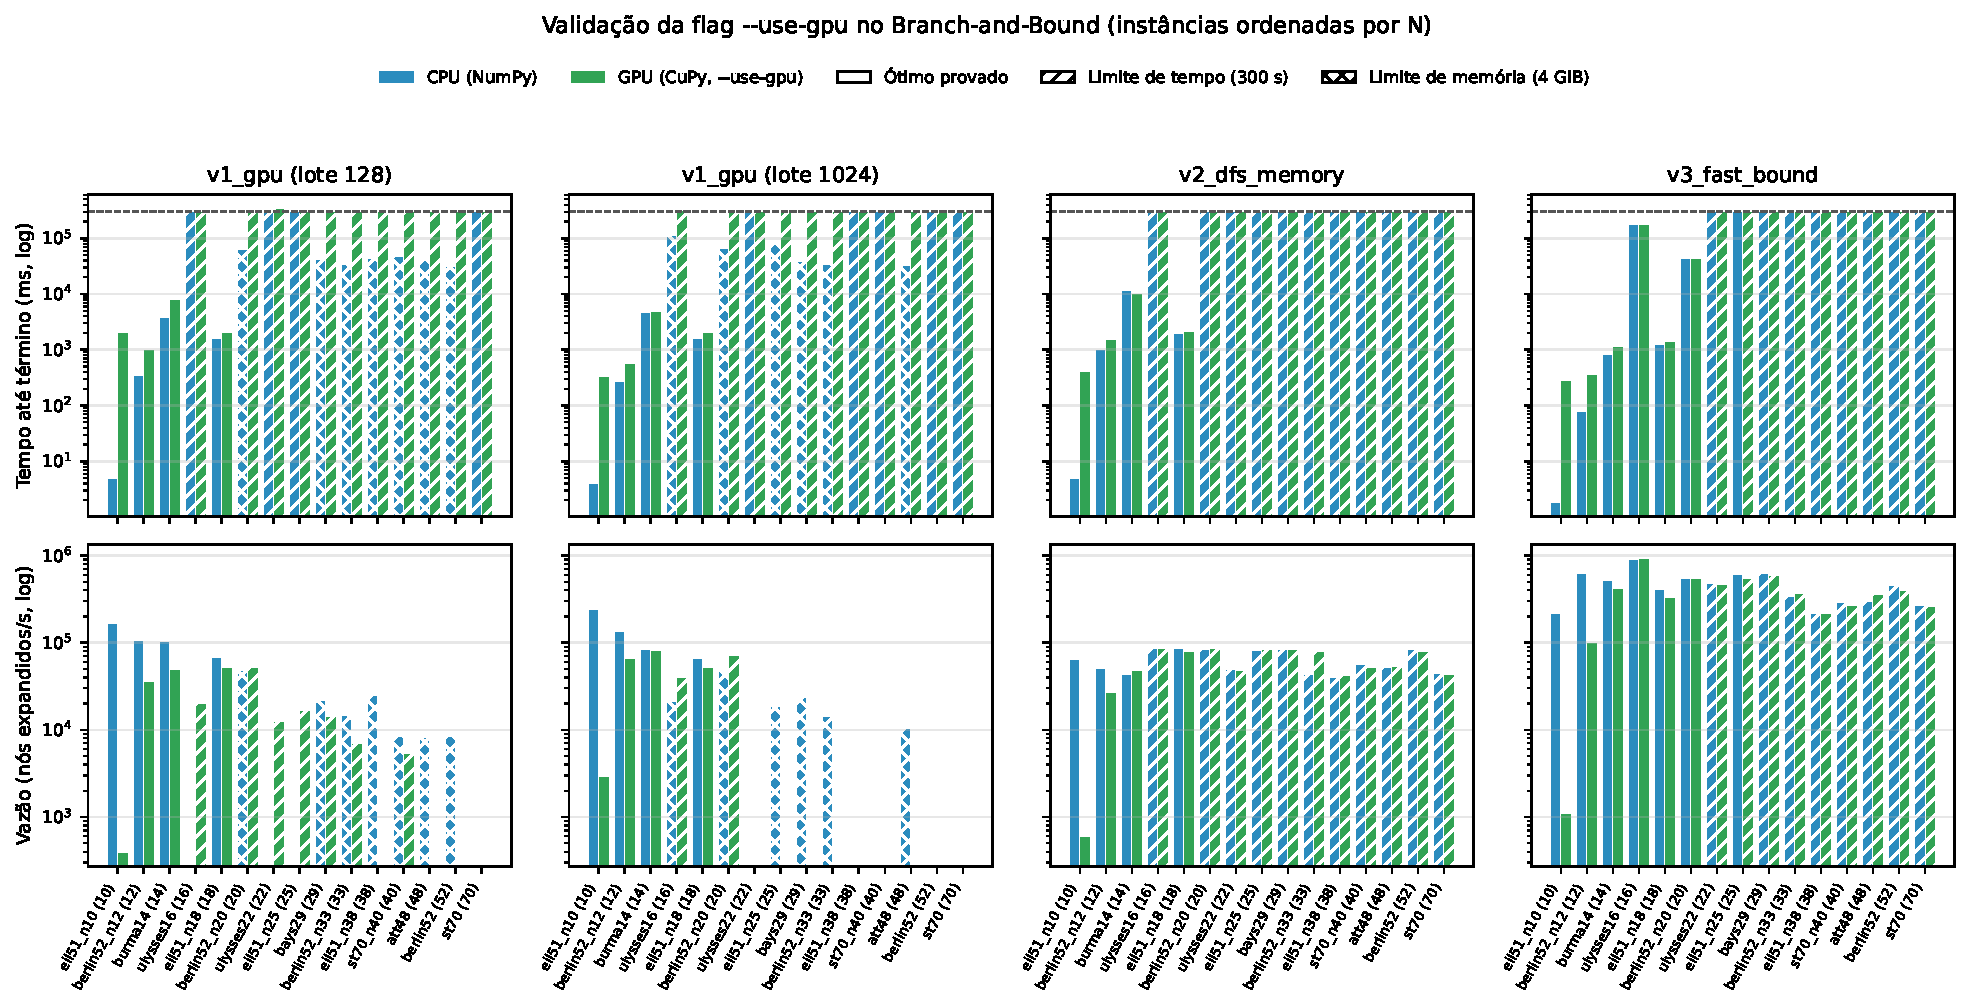
\includegraphics[width=\linewidth]{figures/fig6_gpu_validation.pdf}%
  }{\todoLab{Figura 6 ainda não gerada}}
  \caption{Bateria D. Tempo até o término (acima) e vazão em nós expandidos por segundo
  (abaixo), em CPU e GPU, para cada configuração. Instâncias ordenadas por $N$.}
  \label{fig:gpu}
\end{figure}
